\section{Methodology}
\label{sec:methodology}

We propose a soft-coded MXFP4 training framework as a plug-in extension to Transformer Engine’s blockwise FP8 recipe. FP4 elements are stored via bit-level packing into \texttt{uint8} containers. As illustrated in Figure~\ref{fp4flow}, our approach introduces a hybrid-precision dataflow designed to balance throughput with numerical stability.

Specifically, during the forward pass, activations are quantized into MXFP4 immediately before the All-to-All (A2A) dispatch to reduce communication volume, while the combine phase retains BF16 accumulation to preserve reduction accuracy. In addition, activation replicas required for recomputation are cached in MXFP4 format, significantly reducing the activation memory footprint.

In the backward pass, we intentionally revert to the standard FP8 communication and storage flow. Empirical profiling shows that the additional dequantization overhead introduced by FP4 (e.g., FP4 $\rightarrow$ FP8) outweighs potential communication savings for gradients. This asymmetric design—aggressive FP4 usage in the forward pass and conservative precision in the backward pass—achieves favorable end-to-end performance without compromising convergence.


To realize this flow efficiently, we develop specialized kernels---\texttt{BF16ToFP4Row}, \texttt{FP4RowToFP8Row}, and \texttt{FP4RowToFP8Col}---that perform layout-aware conversions bridging FP4 storage and FP8 computation.

\paragraph{Notation.}
Given FP4-quantized tensors with 4-bit values $X_{\mathrm{fp4}}$ and scaling factors $\mathrm{SF}_{\mathrm{fp4}}$, our conversion algorithm proceeds as follows. Hereafter, we use \textbf{SF} to denote scaling factor, \textbf{sign} for the sign bit, \textbf{exp} for exponent, and \textbf{mant} for mantissa. For clarity, scaling factors and sign bits are denoted using distinct symbols throughout. We use C-style bitwise operators throughout the paper. 



\begin{figure*}[t]
  \centering
  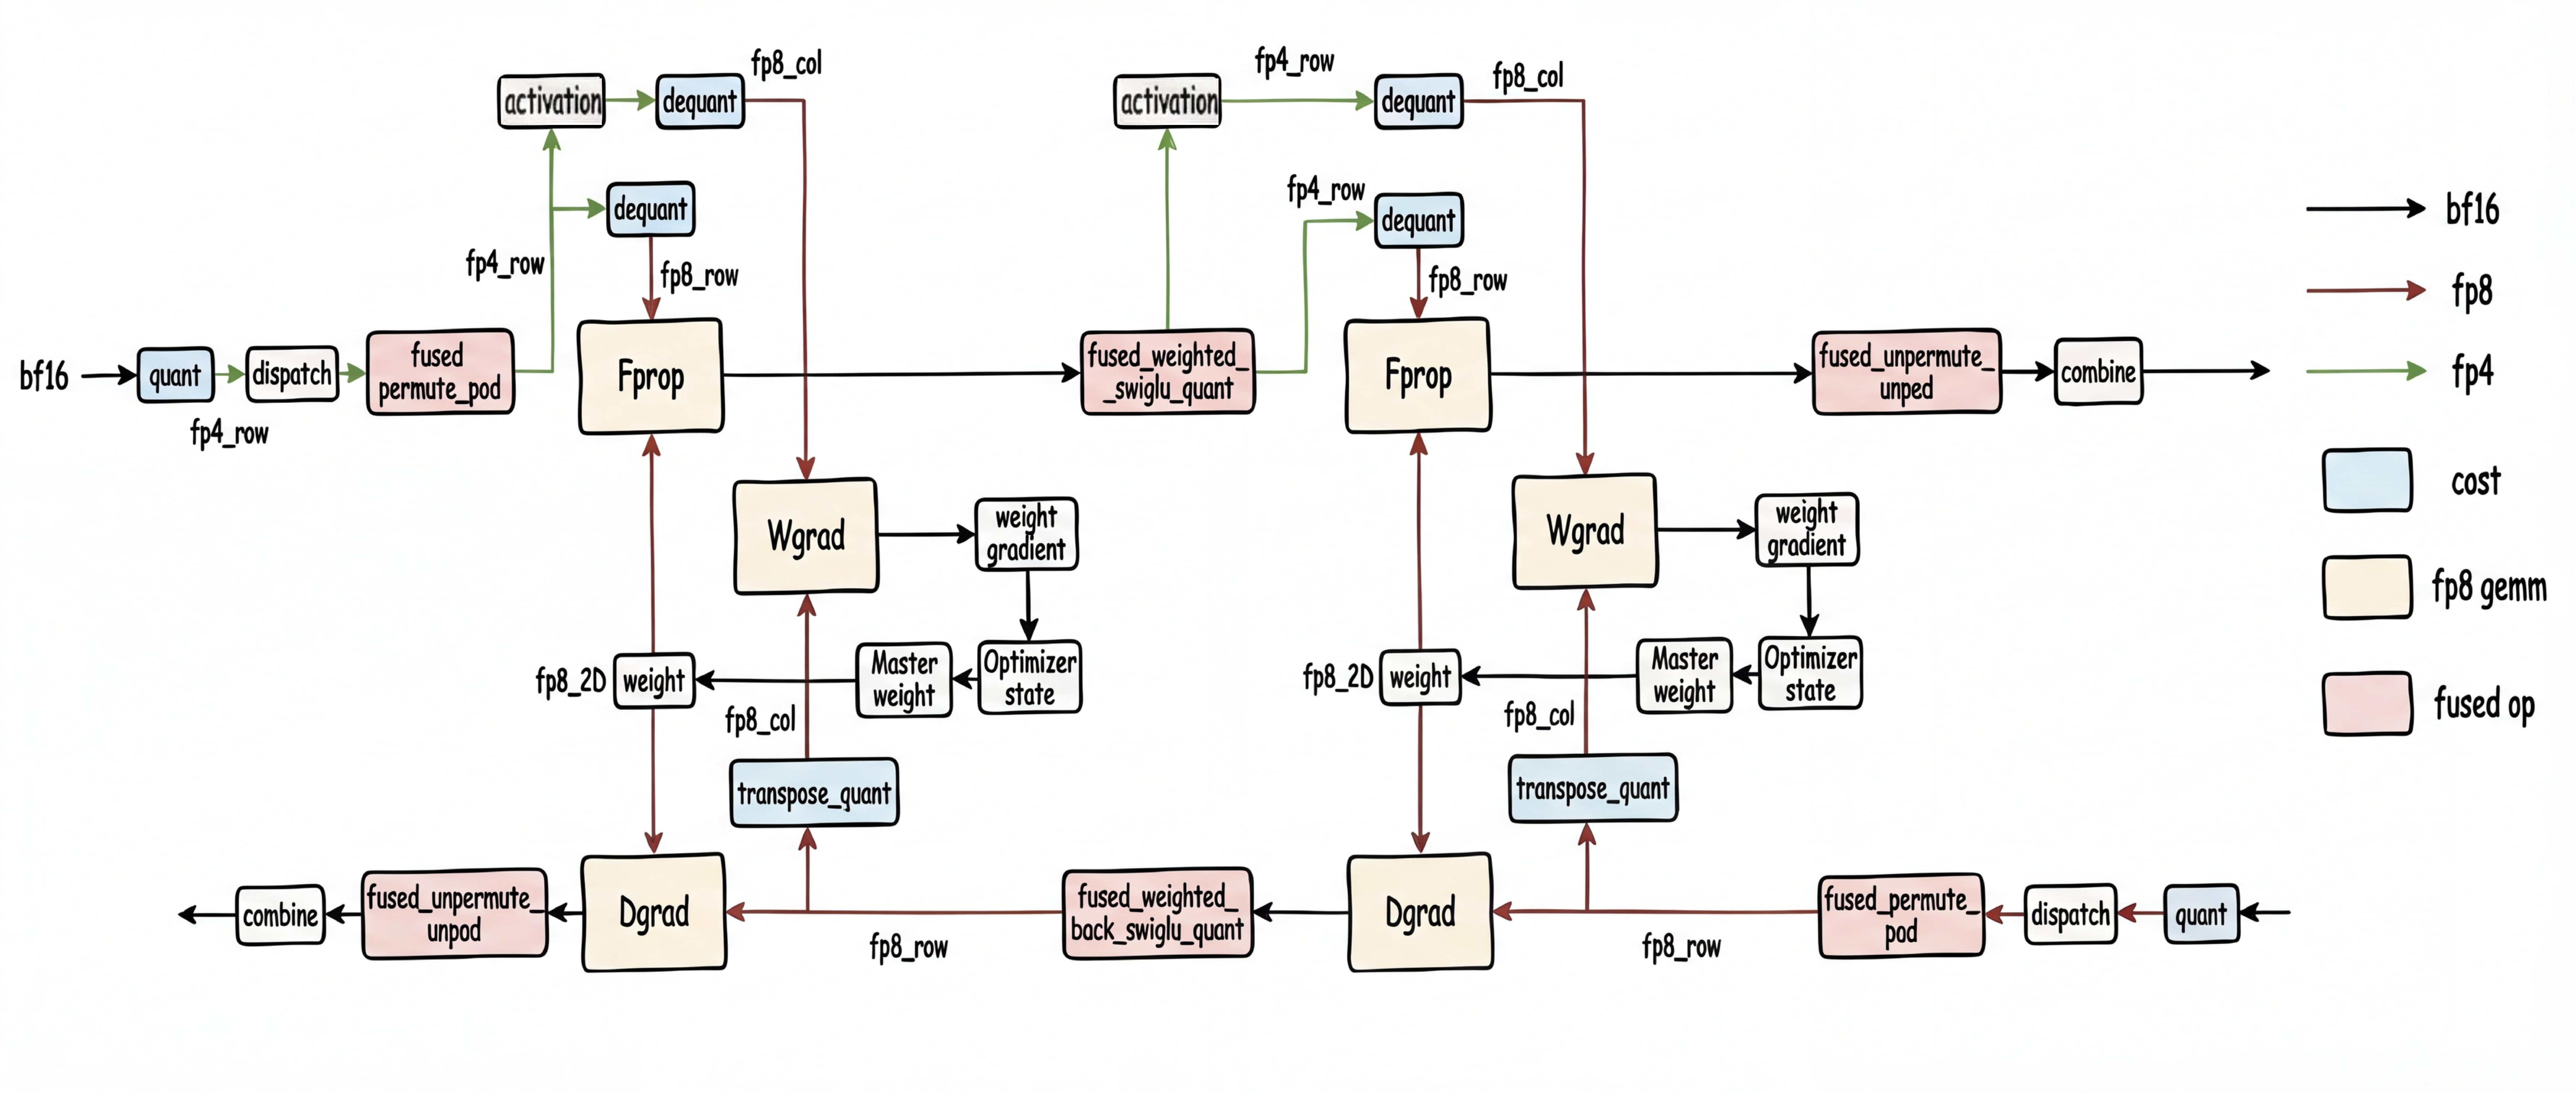
\includegraphics[scale=0.1]{images/fp4flow_opt4_compress.pdf}
%  \caption{FP4 flow.}
    \caption{Overview of the MXFP4 hybrid-precision training flow.}
  \label{fp4flow}
\end{figure*}

\subsection{MXFP4 Quantization Specification on Non-Native Hardware}

%MXFP4 is a standardized numerical format defined by the Open Compute Project (OCP). A core architectural property of MXFP4 is its micro-scaling framework, which adopts a block-based quantization strategy with a fixed granularity of $1 \times 32$ elements. Compared to coarse-grained methods such as per-tensor or per-row scaling, MXFP4 provides finer granularity and a higher density of scaling factors.
In MXFP4, each block of 32 elements shares a common power-of-two scale factor and uses a 4-bit floating-point encoding with one sign bit, two exponent bits, and one mantissa bit (E2M1). This block-wise microscaling quantization achieves finer granularity than coarse per-tensor or per-row scaling schemes and has been shown to improve quantization fidelity and dynamic range in practice~\cite{ocp_mx_specification, micro_quant_arxiv}.

%For a standard floating-point number (e.g., IEEE~754), the numerical value $V$ is defined as $V = (-1)^{\mathrm{sign}} \cdot 1.\mathrm{mant} \times 2^{\mathrm{exponent}}$. In this formulation, the mantissa is typically normalized to the range $[1, 2)$ and takes the form $1.m$, where $m$ denotes the fractional bits. MXFP4 is a specialized instance of this representation, consisting of a 1-bit sign, a 2-bit exponent, and a 1-bit mantissa. When the exponent bits take their minimum value (i.e., all zeros), the representation no longer uses the implicit leading bit and instead directly encodes the mantissa. This regime corresponds to denormal numbers, defined as $V = (-1)^{\mathrm{sign}} \times 0.\mathrm{mant} \times 2^{\mathrm{exponent}}$. In this case, the exponent is treated as a constant offset used to shift the representable range. For denormal values, the effective exponent is fixed at the minimum representable value, typically defined as the bias minus one.
%MXFP4 follows the standard sign--exponent--mantissa representation used in IEEE~754 floating-point formats, but with an \texttt{E2M1} layout consisting of a 1-bit sign, a 2-bit exponent, and a 1-bit mantissa. When the exponent reaches its minimum value, MXFP4 enters a denormal regime in which the implicit leading bit is dropped and the mantissa is encoded directly, extending the representable dynamic range at the cost of mantissa precision. In this regime, the effective exponent is fixed to the minimum representable value (i.e., bias minus one).
The underlying floating-point representation in MXFP4 follows the sign–exponent–mantissa convention of IEEE 754 formats. A real value is typically encoded with an implicit leading mantissa bit when the exponent is above its minimum; when the exponent bits are all zeros, values enter the subnormal (denormal) regime, where the implicit leading bit is dropped and the mantissa directly encodes fractional magnitude. Subnormal numbers extend dynamic range at the cost of leading precision, consistent with IEEE 754 definitions for small exponents~\cite{ieee754_floating_point}.


In our software implementation, we prioritize the computation of scaling factors. This design enables asynchronous scale write-backs to overlap with subsequent compute kernels, effectively hiding latency. The scale computation proceeds as follows.

For each $1 \times 32$ block of the input tensor, we determine the maximum absolute value, denoted as $\mathrm{group\_max}$. The floating-point scale is obtained by normalizing this value with respect to the maximum representable integer in MXFP4, denoted as $\mathrm{FP4\_MAX}=6$. Specifically, the intermediate scale is computed as $\mathrm{group\_max} / 6$ and then cast into the UE8M0 format by rounding up to the nearest power of two. Formally, the scaling factor is defined as
\[
\mathrm{SF} = 2^{\left\lceil \log_2 \left( \max(|X_{\mathrm{BF16}}|) / \mathrm{FP4\_MAX} \right) \right\rceil} .
\]
Once the scale factor is computed, quantization proceeds in two stages. First, the input values are numerically mapped and cast from BF16 to the MXFP4 representation. Second, the resulting low-precision values are reorganized via bit-level extraction and packing into \texttt{uint8} containers, ensuring compatibility with the NVIDIA Hopper memory layout and tensor core requirements.

The conversion begins by normalizing each BF16 input value using the corresponding floating-point scale, mapping it into the MXFP4 dynamic range. CUDA intrinsic functions are used to facilitate the casting from floating-point to integer representations. A key consideration in this process is the treatment of subnormal values. When the exponent falls below the minimum representable threshold, the implicit leading bit must be explicitly materialized and subjected to appropriate bit shifting. This mechanism trades mantissa precision for extended dynamic range, implementing gradual underflow.

The kernel implementation relies on two core bitwise operations. First, \emph{materializing the implicit bit}: following the IEEE~754 convention, normalized values contain an implicit leading bit of one. We apply the transformation $(\texttt{0x400000u} \,\texttt{|}\, (\mathrm{mant} \texttt{>>} 1))$, which right-shifts the 23-bit mantissa by one and performs a bitwise OR with \texttt{0x400000u}, explicitly reinserting the hidden bit into the most significant position of the fraction. Second, \emph{exponent alignment via right shifting}: the mantissa is further right-shifted by a computed offset, effectively increasing the exponent until it aligns with the minimum representable range of the target format.

Rounding behavior is another critical aspect of the implementation. For MXFP4, we adopt round-to-nearest, ties-to-even (RTNE). When truncating high-precision values (e.g., FP32 with a 23-bit mantissa) to ultra-low precision formats, naive truncation introduces systematic bias. RTNE, as the default rounding mode in IEEE~754, ensures that quantization error remains statistically zero-centered.

The rounding decision is derived from three signals: the last bit ($L$), the guard bit ($G$), and the sticky bit ($S$). Here, $L$ denotes the least significant bit of the target format (bit~22), where $L=1$ indicates an odd value and $L=0$ an even value. The guard bit $G$ corresponds to the first bit beyond the target precision (bit~21) and indicates whether the remainder is at least $0.5$. The sticky bit $S$ is defined as the logical OR of all remaining lower-order bits (bits~20--0). The final rounding increment is determined by
$R = G \,\&\, (S \,|\, L)$.

After consolidating the sign, exponent, and mantissa fields of the MXFP4 representation, two FP4 values are packed into a single \texttt{uint8} element. This final step consists of standard bit-manipulation and packing operations, which we omit for brevity.

\subsection{Loss-Neutral FP4-Enabled Mixed Precision Training Flow}

A key design choice is to place quantization immediately before the All-to-All (A2A) dispatch. FP4-quantized activations are packed into \texttt{uint8} containers, reducing both communication volume and memory footprint without altering the core computation logic. As a result, the framework remains fully compatible with existing FP8-based hardware acceleration pipelines.

\textbf{Quantization Timing and Communication Optimization.}
Strictly positioning quantization prior to A2A dispatch enables a substantial reduction in communication payload. Specifically, the standard FP8 communication format—consisting of FP8 activations with FP32 scaling factors—is replaced by a compact representation that combines packed FP4 activations with 8-bit integer scales.

Assuming an activation tensor of shape $M \times K$, the communication footprint can be analyzed as follows. In the FP8 baseline, activations are transmitted as \texttt{uint8} values, incurring $M \cdot K$ bytes, while scaling factors are stored as FP32 with a block size of 128, contributing an additional $(M \cdot K / 128) \cdot 4$ bytes. This results in a total payload of approximately $1.03 \cdot M \cdot K$ bytes. In contrast, under MXFP4, two FP4 values are packed into a single \texttt{uint8} byte, reducing the activation payload to $(M \cdot K)/2$ bytes. Scaling factors follow the MXFP4 specification and are stored as 8-bit integers with a block size of 32, contributing $(M \cdot K / 32) \cdot 1$ byte. The total communication volume is therefore approximately $0.53 \cdot M \cdot K$ bytes, corresponding to a reduction of roughly 50\%.

We implement this customized data flow within the DeepEP communication library by extending the A2A operator to support packed FP4 formats. Throughout this process, the quantization and de-quantization steps are designed to remain logically lossless with respect to the original FP8 computation.

\textbf{Decoupling Computation and Storage Precision.}
To balance computational throughput and memory efficiency, we adopt a decoupled precision strategy. All forward and backward GEMM operations are executed in FP8, allowing us to fully leverage native Tensor Core acceleration and preserve numerical stability. In contrast, activation tensors produced during the forward pass are immediately quantized and cached in HBM as MXFP4 replicas. Compared to FP8 activation caching, this strategy reduces activation memory usage by nearly 50\%, enabling larger batch sizes, more aggressive recomputation strategies, or further model scaling.

\textbf{Specialized Kernel Support.}
Supporting this hybrid-precision flow requires layout-aware format conversion. We therefore develop three specialized CUDA kernels. \texttt{BF16ToFP4Row} performs row-wise MXFP4 quantization and packing during the forward pass. \texttt{FP4RowToFP8Row} efficiently de-quantizes packed FP4 activations into FP8 row-major format for standard GEMM execution. Finally, \texttt{FP4RowToFP8Col} is designed for weight-gradient (Wgrad) computation, where a transposed view of the activation tensor is required. This kernel fuses de-quantization with matrix transposition, directly converting FP4 row-major storage into FP8 column-major format to minimize memory traffic.

\textbf{Strategic Fallback in Backward Propagation.}
Although FP4 provides significant storage and communication benefits, applying it uniformly across all training stages introduces trade-offs. Our profiling shows that, in the backward pass, the overhead of additional de-quantization steps (e.g., BF16 $\rightarrow$ FP4 $\rightarrow$ FP8) outweighs the potential communication savings for gradients. Consequently, we intentionally revert to a standard FP8 communication flow during backpropagation. This asymmetric design—aggressive FP4 usage in the forward pass and conservative precision in the backward pass—proves effective in optimizing end-to-end training throughput without compromising convergence.


\subsection{Direct FP4-to-FP8 Conversion Algorithm}

While NVIDIA Hopper GPUs provide efficient hardware support for FP8 matrix multiplication, they lack native instructions for FP4 computation. As a result, the efficiency of our approach critically depends on an optimized conversion pipeline that bridges storage-efficient MXFP4 representations and compute-efficient FP8 operands.

A direct conversion is non-trivial due to the structural mismatch between MXFP4 and FP8 formats. MXFP4 uses an \texttt{E2M1} encoding packed into \texttt{uint8} containers, with a block size of 32 and scaling factors stored in UE8M0 format. In contrast, FP8 adopts an \texttt{E4M3} layout with a block size of 128 and FP32 scaling. A naive conversion path that up-casts MXFP4 to BF16 and subsequently down-casts to FP8 (FP4 $\rightarrow$ BF16 $\rightarrow$ FP8) incurs substantial latency and memory overhead.

To avoid these costs, we propose a direct bit-wise FP4-to-FP8 conversion algorithm that bypasses the BF16 intermediate. The algorithm combines integer-domain format remapping with a hierarchical scaling alignment strategy to reconcile differences in mantissa layout, exponent bias, and block granularity. Algorithm~\ref{alg:DirectConversion} summarizes the complete FP4-to-FP8 conversion procedure.

\textbf{Bit-wise Format Remapping.}
The conversion begins by unpacking the sign, exponent, and mantissa fields from the FP4 bitstream. The exponent is adjusted directly in the integer domain according to
\[
E_{\text{fp8}} = E_{\text{fp4}} - \mathrm{Bias}_{\text{fp4}} + \mathrm{Bias}_{\text{fp8}}.
\]
The single-bit mantissa of the FP4 \texttt{E2M1} format is then left-shifted to align with the most significant bit of the FP8 \texttt{E4M3} mantissa field. This operation preserves relative precision while avoiding floating-point arithmetic during format conversion.

\textbf{Hierarchical Scaling Alignment.}
The primary challenge arises from the mismatch in block granularity: four MXFP4 blocks of 32 elements must be mapped onto a single FP8 block of 128 elements. We address this using a max-based hierarchical alignment strategy.

First, a target scale $S_{\text{target}}$ is selected as the maximum scaling factor among the four source MXFP4 blocks. Second, to preserve numerical equivalence, each element’s exponent is compensated by the difference between the local block scale and the target scale,
\[
E'_{\text{fp8}} = E_{\text{fp8}} - (S_{\text{target}} - S_{\text{sub}}).
\]
To mitigate underflow when the disparity between local and global scales is large, we introduce a small empirically chosen shift constant $\delta$, which is folded into the target scale selection during implementation.

Finally, because MXFP4 scaling factors are stored in UE8M0 format and represent exact powers of two, we map each 8-bit scale directly into the exponent field of an FP32 value via bit shifting. This avoids costly floating-point exponentiation and ensures hardware-efficient casting.


\begin{algorithm}[!hbtp]
    \caption{Direct FP4-to-FP8 Conversion Algorithm}
    \label{alg:DirectConversion}
    \renewcommand{\algorithmicrequire}{\textbf{Input:}}
    \renewcommand{\algorithmicensure}{\textbf{Output:}}
    
    \begin{algorithmic}[1]
        \REQUIRE $X_{\text{fp4}} (X_0 \sim X_3)$, $\mathrm{SF}_{\text{fp4}} (\mathrm{SF}_0 \sim \mathrm{SF}_3)$
        \ENSURE $X_{\text{fp8}}$, $\mathrm{SF}_{\text{fp8}}$
        
        \STATE $\mathrm{SF}_{\text{fp8}} = \max(\mathrm{SF}_{\text{fp4}}) - 6$
        \STATE $E_{i,\text{adjust}} = \mathrm{SF}_{\text{fp8}} - \mathrm{SF}_i$
        \STATE $\text{sign}_i = (X_i \texttt{>>} 3) \ \&\ 1$
        \STATE $E_{i,\text{fp4}} = (X_i \texttt{>>} 1) \ \&\ 3$
        \STATE $M_i = X_i \ \&\ 1$
        \STATE $E_{i,\text{fp8}} = E_{i,\text{fp4}} - \mathrm{Bias}_{\text{fp4}} + \mathrm{Bias}_{\text{fp8}}$
        \STATE $E_i = E_{i,\text{fp8}} - E_{i,\text{adjust}}$
        \STATE $X_{i,\text{fp8}} = (\text{sign}_i \texttt{<<} 7) \mid (E_i \texttt{<<} 3) \mid (M_i \texttt{<<} 2)$
        \STATE $X_{\text{fp8}} = \{X_{0,\text{fp8}} \sim X_{3,\text{fp8}}\}$
        
        \RETURN $X_{\text{fp8}}$, $\mathrm{SF}_{\text{fp8}}$
    \end{algorithmic}
\end{algorithm}

\subsection{High-Performance Kernel Implementation}

We implement a suite of highly optimized CUDA kernels for the FP4-enabled training pipeline. In particular, for weight gradient computation (Wgrad), which requires a transposed view of the activation tensor, we design a fused \texttt{FP4RowToFP8Col} kernel that integrates multiple optimizations to minimize memory traffic and conversion overhead.

\textbf{Operator fusion and layout transformation.}
Conventional implementations perform format conversion and memory layout transformation (i.e., transposition) as separate steps, incurring multiple global memory reads and writes. Our kernel instead fuses de-quantization, matrix transposition, and re-quantization into a single execution unit. By carrying out the layout transformation entirely within on-chip shared memory, we eliminate intermediate global memory accesses and reduce overall global memory bandwidth consumption by approximately $3\times$ compared to BF16-based baselines.

\textbf{Conflict-free shared memory access.}
To convert row-major FP4 storage into column-major FP8 output, we use shared memory as a transposition buffer. To avoid bank conflicts during column-wise accesses, we introduce padding in the shared memory tile, allocating it with a stride of \texttt{[TILE\_DIM][TILE\_DIM + 1]}. This skewed layout ensures that column-wise accesses map to distinct memory banks, enabling full utilization of the shared memory bandwidth.

\textbf{Bit-level arithmetic optimization.}
We exploit the bit-level structure of the MXFP4 and FP8 formats to avoid costly floating-point operations whenever possible: (i) \emph{Scale decoding.} MXFP4 scaling factors stored in UE8M0 format are decoded directly into BF16 by bit shifting (e.g., \texttt{val \texttt{<<} 7}), avoiding floating-point multiplication. (ii) \emph{Power-of-two alignment.} To conform with the scaling conventions used in Transformer Engine, we implement a bit-wise scaling procedure. Instead of computing $2^{\lceil \log_2(x) \rceil}$ via math library calls, we directly manipulate the exponent field of the IEEE~754 representation, significantly reducing instruction latency.

\textbf{Format-compatible expert parallel communication.} 
To support MXFP4 scales stored in compact integer representations (e.g., UE8M0), we generalize scale handling in the expert dispatch path to be byte-addressable and precision-agnostic. Specifically, we propagate the scale element size across intranode and internode communication, RDMA/NVL buffer layout, and kernel copy logic, so that scale payloads are treated as variable-sized byte regions rather than implicitly assumed FP32 tensors. This generalization is reflected in per-token communication footprint computation, clean-metadata derivation, and symmetric buffer offset calculation, eliminating buffer over-allocation and misalignment when integer-encoded scales are used. At the kernel level, scale transfers dynamically select between FP32 and byte-wise copy paths based on the propagated element size, while preserving alignment constraints required by TMA and warp-level copy mechanisms.

\textbf{Native support for ragged MoE tensors.}
In Mixture-of-Experts architectures, the number of tokens routed to each expert varies dynamically, resulting in ragged tensors. Our kernel natively supports variable-length splits through precomputed offsets (\texttt{split\_lens}, \texttt{split\_offsets}), dynamically computing output addresses for contiguous storage without padding. Vectorized stores are employed even on misaligned boundaries, with edge cases handled entirely within registers.

See Appendix~\ref{sec:appendix-code} for implementation details and code integration instructions.